\documentclass[12pt,a4paper]{amsart}
\usepackage[slovene]{babel}
\usepackage[utf8]{inputenc}
\usepackage{amsmath,amssymb,amsfonts}
\usepackage{url}
\usepackage[dvipsnames,usenames]{color}
\usepackage{graphicx}
\usepackage{listings}

\newcommand{\program}{FINANČNA MATEMATIKA}
\newcommand{\ime}{Brina Ribič, David Rozman}
\newcommand{\naslovdela}{Naključni sprehodi v lizikah}
\newcommand{\letnica}{2022}

\begin{document}
    
\begin{center}
    \thispagestyle{empty}
\noindent{\large
UNIVERZA V LJUBLJANI\\[1mm]
FAKULTETA ZA MATEMATIKO IN FIZIKO\\[5mm]
\program\ -- 1.~stopnja}
\vfill
\end{center}


\begin{center}
{\bf \naslovdela}\\[10mm]
Poročilo\\[1cm]
\end{center}
\vfill

\begin{center}
    Avtorja: {\large
\ime}\\[2mm]
   \noindent{\large
Ljubljana, \letnica} 
\end{center}
\pagebreak

\tableofcontents
\newpage

\section{Uvod}
V tem poročilu bova predstavila rezultate projektne naloge 'Naključni sprehodi v lizikah'. Najprej bova predstavila
problem ter kako sva se ga lotila, nato pa prikazala rezultate analize z grafi in tabelami.

\section{Opis problema}
Graf v obliki lizike je podan s parom $(m,n)$, kjer $m$ predstavlja število vozlišč polnega grafa, $n$ pa število
vozlišč na grafu poti. Da dobimo graf lizike, oba grafa povežemo z mostom. Po grafu opravimo naključni sprehod. V 
odvisnosti od parametrov $m$ in $n$ so naju zanimali sledeči pričakovani časi:
\begin{itemize}
    \item Pričakovani čas, da obiščemo vsa vozlišča v grafu (Čas pokritja)
    \item Pričakovani čas, da pridemo od enega v drugo vozlišče (Čas dosega)
    \item Pričakovani čas, da se vrnemo v začetno vozlišče (Čas vrnitve)
\end{itemize}
Zanimalo naju je tudi, kaj se zgodi s pričakovanim časom, če graf malce spremeniva, na primer dodava na drugi konec
poti še en poln graf itd.

\begin{figure}[h]
    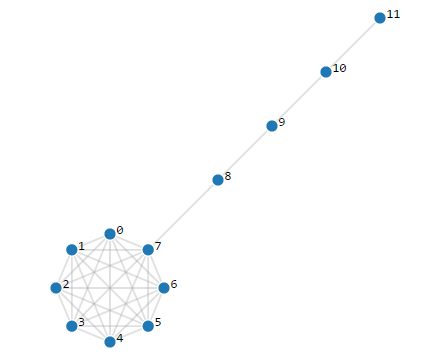
\includegraphics[width=\textwidth]{Lollipop_graph.png}
    \caption{Graf lizike (8,4)}
\end{figure}

\section{Potek reševanja}
Za reševanje problema sva uporabila programski jezik Python. Najprej sva napisala funkcije, ki zgenerirajo želeni graf.
Kot argument sprejmejo število vozlišč, vrnejo pa slovar, kjer ključi predstavljajo vozlišča, vrednosti so pa seznami
sosednjih vozlišč. Nato sva sestavila funkcije, ki po grafu opravijo naključni sprehod. Delujejo na sledeč način: 
Postavimo se v začetno vozlišče. Na vsakem koraku se premaknemo v naključno sosedno vozlišče, ki ga poberemo iz
seznama sosedov. Postopek ponavljamo dokler določen pogoj ni izpolnjen (npr. trenutno vozlišče je enako začetnemu,
če nas zanima čas vrnitve). Nazadnje sva definirala še funkcije, ki opravijo želeno število ponovitev naključnih sprehodov
in vrnejo povprečni čas. Sledi zgled funkcije, ki zgenerira pot z  $n$ vozlišči.


Za vsak tip povprečnega časa, ki sva ga želela analizirati, sva naredila ustrezno veliko število ponovitev poskusov v
za več parametrov $m$ in $n$. Iz tabel in grafov sva nato poskusila ugotoviti časovno zahtevnost.

\section{Navaden graf lizike}

Najprej si bomo pogledali analizo navadnega grafa lizike, sestavljenega iz klike z $m$ vozlišči, poti z $n$ vozlišči in
mosta.

\subsection{Čas pokritja}

Da dobimo pravi čas pokritja, si moramo izbrati primerno začetno vozlišče. Z malo razmisleka hitro ugotovimo, da je
za najdaljši čas sprehoda po celotnem grafu potrebno začeti v vozlišču na kliki, ki ni del mostu, kajti tako, da bo
trajalo najdlje časa, da pridemo do konca poti, ki je najtežje dosegljivi del grafa.

Sledeča tabela prikazuje pričakovani čas pokritja glede na parametre $m$ in $n$. Za vsak primer sva izvedla 100.000
naključnih sprehodov in za pričakovani čas vzela njihovo povprečje.

\begin{table}[!ht]
    \centering
    \begin{tabular}{|l|l|l|l|l|l|l|l|l|l|}
    \hline
        m-n & 2 & 3 & 4 & 5 & 6 & 7 & 8 & 9 & 10 \\ \hline
        3 & 19 & 30 & 43 & 59 & 76 & 96 & 116 & 139 & 165 \\ \hline
        4 & 32 & 49 & 68 & 90 & 113 & 139 & 165 & 195 & 226 \\ \hline
        5 & 49 & 74 & 102 & 131 & 162 & 195 & 230 & 267 & 307 \\ \hline
        6 & 71 & 105 & 142 & 182 & 222 & 265 & 311 & 359 & 410 \\ \hline
        7 & 96 & 143 & 193 & 243 & 296 & 351 & 407 & 467 & 528 \\ \hline
        8 & 125 & 186 & 248 & 313 & 381 & 452 & 520 & 594 & 667 \\ \hline
        9 & 158 & 235 & 314 & 394 & 479 & 564 & 651 & 741 & 836 \\ \hline
        10 & 196 & 290 & 386 & 485 & 588 & 690 & 799 & 904 & 1009 \\ \hline
    \end{tabular}
\end{table}

Opazimo, da povečanje parametra $m$ bolj vpliva na pričakovani čas kot povečanje parametra $n$. To je zato, ker 
ima vsako vozlišče v kliki veliko povezav in traja veliko časa, da bomo obiskali vsa, medtem ko imamo na poti vedno
največ 2 izbiri za naslednje vozlišče.

Na naslednjih grafih vidimo kako povečanje določenega parametra vpliva na pričakovani čas. Prva trojica prikazuje
spreminjanje časa pri fiksnem $m$ in naraščajočim $n$, v drugi trojici pa sta vlogi zamenjani.

\begin{figure}[h]
    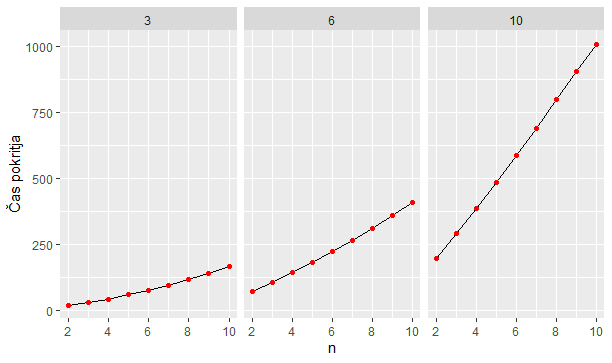
\includegraphics[width=\textwidth]{Rplot.png}
\end{figure}

\begin{figure}[h]
    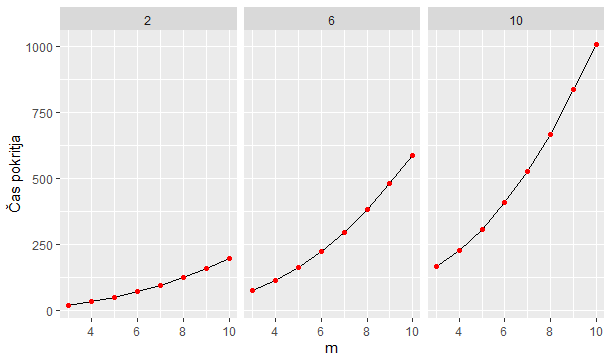
\includegraphics[width=\textwidth]{fiksenn.png}
\end{figure}

Vidimo, da se z $n$-jem pričakovani čas povečuje skoraj linearno, z $m$-jem pa rahlo kvadratično. Če si še ogledamo
vrednosti v tabeli, hitro opazimo, da je pričakovani čas pri nekem $m$ in $n$ vedno blizu $m^2n$. Tako smo pokazali,
da je pričakovani čas sprehoda po grafu lizike $\mathcal{O}(m^2n)$.

Tu bi poudarili še pomembnost začetne izbire vozlišča. Enak eksperiment sva izvedla še z začetkom v vozlišču na koncu
poti. Naslednja tabela prikazuje, kako se pričakovani čas pokritja spremeni, če si izberemo napačno začetno vozlišče.

\begin{table}[!ht]
    \centering
    \begin{tabular}{|l|l|l|l|l|l|l|l|l|l|}
    \hline
        m-n & 2 & 3 & 4 & 5 & 6 & 7 & 8 & 9 & 10 \\ \hline
        3 & 10 & 16 & 25 & 36 & 48 & 64 & 80 & 98 & 119 \\ \hline
        4 & 12 & 18 & 27 & 37 & 49 & 64 & 80 & 99 & 119 \\ \hline
        5 & 14 & 21 & 29 & 39 & 51 & 65 & 82 & 100 & 120 \\ \hline
        6 & 17 & 23 & 31 & 41 & 54 & 68 & 84 & 102 & 122 \\ \hline
        7 & 20 & 26 & 34 & 44 & 56 & 70 & 86 & 104 & 124 \\ \hline
        8 & 23 & 29 & 37 & 47 & 59 & 73 & 89 & 107 & 127 \\ \hline
        9 & 27 & 33 & 41 & 50 & 62 & 76 & 92 & 110 & 130 \\ \hline
        10 & 30 & 36 & 44 & 54 & 65 & 79 & 95 & 113 & 132 \\ \hline
    \end{tabular}
\end{table}

Ker smo začeli v težko dosegljivem vozlišču smo hitro prehodili celotno pot, ostala pa je le še klika, ki smo jo hitro
prehodili. Opazimo, da v tem primeru sprememba $m$ zelo malo vpliva na čas pokritja.

\subsection{Čas dosega}

Sedaj si bomo pogledali pričakovane čase, da pridemo iz enega vozlišča v drugo.

\subsubsection{Vozlišča v kliki}

Kot prvo bi si pogledali potreben čas, da pridemo iz enega vozlišča v polnem grafu do drugega. Ločili bomo dva primera:
\begin{itemize}
    \item Začetno vozlišče je del mostu
    \item Začetno in končno vozlišče nista del mostu
\end{itemize}
Če bi za končno vozlišče izbrali vozlišče pri mostu, bi dobili navaden čas dosega za poln graf. Če pa za končno
vozlišče vzamemo neko drugo vozlišče v kliki, s tem dopuščamo, da se med sprehodom znajdemo tudi na poti, kar bo
povečalo pričakovani čas.

Prva tabela prikazuje čas, če je začetno vozlišče del mostu

\begin{table}[!ht]
    \centering
    \begin{tabular}{|l|l|l|l|l|l|l|l|l|l|}
    \hline
        m-n & 2 & 3 & 4 & 5 & 6 & 7 & 8 & 9 & 10 \\ \hline
        3 & 5 & 6 & 7 & 9 & 10 & 11 & 13 & 14 & 15 \\ \hline
        4 & 5 & 6 & 7 & 8 & 9 & 10 & 11 & 12 & 13 \\ \hline
        5 & 6 & 6 & 7 & 4 & 9 & 10 & 10 & 11 & 12 \\ \hline
        6 & 6 & 7 & 8 & 8 & 9 & 10 & 10 & 11 & 12 \\ \hline
        7 & 7 & 7 & 8 & 9 & 9 & 10 & 10 & 11 & 12 \\ \hline
        8 & 8 & 8 & 9 & 9 & 10 & 10 & 11 & 11 & 12 \\ \hline
        9 & 9 & 9 & 10 & 10 & 11 & 11 & 12 & 12 & 12 \\ \hline
        10 & 10 & 10 & 11 & 11 & 11 & 12 & 12 & 13 & 13 \\ \hline
    \end{tabular}
\end{table}

Hitro opazimo zanimivost in sicer, da se je pri majhnih $m$ s povečanjem tega parametra čas dosega celo zmanjšal. Razlog
je v tem, da smo s povečanjem števila povezav v začetnem vozlišču zmanjšali verjetnost, da se bomo na začetku sprehoda
premaknili na pot, torej stran od ciljnega vozlišča. Pri majhnih $m$ torej dolžina poti precej bolj vpliva na čas kot pri
velikih, kjer je verjetnost, da se bomo na njej znašli precej majhna.

Druga tabela prikazuje čas, če začetno vozlišče ni del mostu.

\begin{table}[!ht]
    \centering
    \begin{tabular}{|l|l|l|l|l|l|l|l|l|l|}
    \hline
        m-n & 2 & 3 & 4 & 5 & 6 & 7 & 8 & 9 & 10 \\ \hline
        3 & 3 & 4 & 5 & 5 & 6 & 7 & 7 & 8 & 9 \\ \hline
        4 & 4 & 5 & 5 & 5 & 6 & 6 & 7 & 8 & 8 \\ \hline
        5 & 5 & 5 & 6 & 6 & 6 & 7 & 7 & 8 & 8 \\ \hline
        6 & 6 & 6 & 6 & 7 & 7 & 7 & 8 & 8 & 8 \\ \hline
        7 & 7 & 7 & 7 & 7 & 8 & 8 & 8 & 9 & 9 \\ \hline
        8 & 8 & 8 & 8 & 8 & 9 & 9 & 9 & 9 & 10 \\ \hline
        9 & 8 & 9 & 9 & 9 & 9 & 10 & 10 & 10 & 10 \\ \hline
        10 & 9 & 10 & 10 & 10 & 10 & 10 & 11 & 11 & 11 \\ \hline
    \end{tabular}
\end{table}

Vidimo, da je večja razlika v primerjavi s prejšnjo tabelo opazna le pri majhnih $m$. Ker je $m$ majhen, je velika
verjetnost, da do vozlišča ob mostu sploh ne bomo prišli, zaradi česar je tu čas dosega manjši. Zaradi podobnih 
razlogov kot prej, da se pri majhnih $m$ vpliv povečanja dolžine poti pozna precej bolj, kot za večje $m$. 

Da bi določili čas dosega v odvisnosti od $m$ in $n$, moramo upoštevati le čase za velike vrednosti teh parametrov.
S prvim parametrom čas očitno raste linearno, drugi pa prispeva zelo malo. Čas dosega je približno
$\mathcal{O}(m+log(n))$.

\subsubsection{Od vrha do dna}

Tu bomo za začetno vozlišče vzeli vozlišče v kliki, ki ni del mostu, za končno pa konec poti, torej najbolj
oddaljeno vozlišče. Rezultate simulacije prikazuje naslednja tabela.

\begin{table}[!ht]
    \centering
    \begin{tabular}{|l|l|l|l|l|l|l|l|l|l|}
    \hline
        m-n & 2 & 3 & 4 & 5 & 6 & 7 & 8 & 9 & 10 \\ \hline
        3 & 18 & 29 & 42 & 57 & 74 & 93 & 114 & 136 & 162 \\ \hline
        4 & 31 & 48 & 67 & 88 & 111 & 164 & 164 & 192 & 223 \\ \hline
        5 & 48 & 73 & 100 & 129 & 159 & 193 & 228 & 265 & 305 \\ \hline
        6 & 69 & 104 & 141 & 180 & 221 & 265 & 309 & 357 & 404 \\ \hline
        7 & 93 & 141 & 189 & 239 & 293 & 348 & 406 & 466 & 528 \\ \hline
        8 & 122 & 185 & 246 & 311 & 379 & 448 & 518 & 591 & 669 \\ \hline
        9 & 155 & 234 & 313 & 394 & 476 & 560 & 647 & 736 & 828 \\ \hline
        10 & 193 & 288 & 386 & 484 & 585 & 688 & 794 & 898 & 1007 \\ \hline
    \end{tabular}
\end{table}

Hitro opazimo, da so vrednosti zelo podobne tistim pri času pokritja. To ni presenetljivo, saj smo v obeh primerih
začeli v istem vozlišču. Čas pa je bil odvisen predvsem od časa dosega konca poti. V tem primeru so vrednosti v 
povprečju malenkost manjše, saj se je sprehod tu vedno ustavil, ko smo dosegli konec poti, pri času pokritja pa 
se je to zgodilo le, če je bilo vozlišče na koncu poti zadnje doseženo, kar pa se ni zgodilo le v redkih primerih.
Čas dosega v tem primeru je torej $\mathcal{O}(m^2n)$

\subsubsection{Od dna do vrha}

Tu bomo zamenjali vlogi vozlišč iz prejšnjega primera. Začeli bomo torej na koncu poti, končali pa v vozlišču na 
kliki, ki ni del mostu. Ker začnemo v najtežje dosegljivem vozlišču, pričakujemo, da bodo pričakovani časi tu precej
krajši.

\begin{table}[!ht]
    \centering
    \begin{tabular}{|l|l|l|l|l|l|l|l|l|l|}
    \hline
        m-n & 2 & 3 & 4 & 5 & 6 & 7 & 8 & 9 & 10 \\ \hline
        3 & 9 & 15 & 23 & 34 & 46 & 60 & 76 & 94 & 115 \\ \hline
        4 & 9 & 15 & 23 & 33 & 45 & 59 & 75 & 93 & 113 \\ \hline
        5 & 10 & 15 & 23 & 33 & 45 & 59 & 74 & 92 & 112 \\ \hline
        6 & 10 & 16 & 24 & 33 & 45 & 59 & 74 & 92 & 112 \\ \hline
        7 & 11 & 17 & 24 & 34 & 45 & 59 & 75 & 92 & 111 \\ \hline
        8 & 12 & 18 & 25 & 35 & 46 & 60 & 76 & 92 & 112 \\ \hline
        9 & 13 & 18 & 26 & 35 & 47 & 60 & 76 & 93 & 112 \\ \hline
        10 & 14 & 19 & 27 & 36 & 47 & 61 & 76 & 93 & 113 \\ \hline
    \end{tabular}
\end{table}

Pričakovanja so se uresničila, časi so tu precej manjši. Ker pot zahteva veliko korakov, da jo prehodimo, je čas tu
odvisen predvsem od njene dolžine. Parameter $m$ tu nima velikega vpliva na čas, saj ko pridemo enkrat v kliko, bomo
hitro dosegli tudi končno vozlišče. Ocenimo, da je čas dosega v tem primeru $\mathcal{O}(n^2+m)$. Da bi pokazala, da 
je to dobra ocena, sva z njo v tabeli vrednosti delila vse izračunane vrednosti.

\begin{table}[!ht]
    \centering
    \begin{tabular}{|l|l|l|l|l|l|l|l|l|l|}
    \hline
        m-n & 2 & 3 & 4 & 5 & 6 & 7 & 8 & 9 & 10 \\ \hline
        3 & 1,286 & 1,250 & 1,211 & 1,214 & 1,179 & 1,154 & 1,134 & 1,119 & 1,117 \\ \hline
        4 & 1,125 & 1,154 & 1,150 & 1,138 & 1,125 & 1,113 & 1,103 & 1,094 & 1,087 \\ \hline
        5 & 1,111 & 1,071 & 1,095 & 1,100 & 1,098 & 1,093 & 1,072 & 1,070 & 1,067 \\ \hline
        6 & 1,000 & 1,067 & 1,091 & 1,065 & 1,071 & 1,073 & 1,057 & 1,057 & 1,057 \\ \hline
        7 & 1,000 & 1,062 & 1,043 & 1,062 & 1,047 & 1,054 & 1,056 & 1,045 & 1,037 \\ \hline
        8 & 1,000 & 1,059 & 1,042 & 1,061 & 1,045 & 1,053 & 1,056 & 1,034 & 1,037 \\ \hline
        9 & 1,000 & 1,000 & 1,040 & 1,029 & 1,044 & 1,034 & 1,041 & 1,033 & 1,028 \\ \hline
        10 & 1,000 & 1,000 & 1,038 & 1,029 & 1,022 & 1,034 & 1,027 & 1,022 & 1,027 \\ \hline
    \end{tabular}
\end{table}

Vidimo, da se z večanjem parametrov količnik res bliža 1, torej hipoteza drži.

\subsection{Čas vrnitve}

Sedaj si bomo pogledali še pričakovani čas, da se pri naključnem sprehodu vrnemo v začetno vozlišče.
Analizirala sva 3 primere začetnih vozlišč:
\begin{itemize}
    \item Vozlišče v kliki, ki ni del mostu
    \item Vozlišče v kliki, ki je del mostu
    \item Vozlišče na koncu poti
\end{itemize}

\subsubsection{Vozlišče v kliki, ki ni del mostu}

Naslednja tabela prikazuje izračunane pričakovane čase.

\newpage

\begin{table}[!ht]
    \centering
    \begin{tabular}{|l|l|l|l|l|l|l|l|l|l|}
    \hline
        m-n & 2 & 3 & 4 & 5 & 6 & 7 & 8 & 9 & 10 \\ \hline
        3 & 5 & 6 & 7 & 8 & 9 & 10 & 11 & 12 & 13 \\ \hline
        4 & 6 & 6 & 7 & 8 & 8 & 9 & 9 & 10 & 10 \\ \hline
        5 & 6 & 6 & 7 & 8 & 8 & 9 & 9 & 10 & 10 \\ \hline
        6 & 7 & 7 & 8 & 8 & 8 & 9 & 9 & 10 & 10 \\ \hline
        7 & 8 & 8 & 8 & 9 & 9 & 9 & 10 & 10 & 10 \\ \hline
        8 & 9 & 9 & 9 & 9 & 10 & 10 & 10 & 11 & 11 \\ \hline
        9 & 10 & 10 & 10 & 10 & 10 & 11 & 11 & 11 & 11 \\ \hline
        10 & 10 & 11 & 11 & 11 & 11 & 12 & 12 & 12 & 12 \\ \hline
    \end{tabular}
\end{table}

Vidimo, da so rezultati zelo podobni časom dosega, ko začetno vozlišče ni bilo del mostu. Ni presenetljivo, saj gre
za zelo podoben tip sprehoda. Pričakovani čas je spet $\mathcal{O}(m+log(n))$.

\subsubsection{Vozlišče v kliki, ki je del mostu}

Sedaj opravimo enak eksperiment, le da obstaja možnost, da se že takoj znajdemo na poti.

\begin{table}[!ht]
    \centering
    \begin{tabular}{|l|l|l|l|l|l|l|l|l|l|}
    \hline
        m-n & 2 & 3 & 4 & 5 & 6 & 7 & 8 & 9 & 10 \\ \hline
        3 & 3 & 3 & 5 & 5 & 6 & 7 & 7 & 8 & 9 \\ \hline
        4 & 4 & 5 & 5 & 6 & 6 & 6 & 7 & 7 & 8 \\ \hline
        5 & 5 & 5 & 6 & 6 & 6 & 7 & 7 & 8 & 8 \\ \hline
        6 & 6 & 6 & 6 & 7 & 7 & 7 & 8 & 8 & 8 \\ \hline
        7 & 7 & 7 & 7 & 7 & 8 & 8 & 8 & 9 & 9 \\ \hline
        8 & 8 & 8 & 8 & 8 & 8 & 9 & 9 & 9 & 9 \\ \hline
        9 & 8 & 9 & 9 & 9 & 9 & 10 & 10 & 10 & 10 \\ \hline
        10 & 9 & 10 & 10 & 10 & 10 & 10 & 11 & 11 & 11 \\ \hline
    \end{tabular}
\end{table}

Rezultati so zelo podobni tistim iz prejšnjega primera, le za malenkost so manjši. Razlog je to, da je to vozlišče
največje stopnje v grafu lizike, zato se lahko hitreje vrnemo vanj.
Pričakovani čas je še vedno $\mathcal{O}(m+log(n))$.

\subsubsection{Vozlišče na koncu poti}

Poglejmo si še, kaj se zgodi, če začnemo na koncu poti.

\begin{table}[!ht]
    \centering
    \begin{tabular}{|l|l|l|l|l|l|l|l|l|l|}
    \hline
        m-n & 2 & 3 & 4 & 5 & 6 & 7 & 8 & 9 & 10 \\ \hline
        3 & 10 & 12 & 14 & 16 & 18 & 20 & 22 & 24 & 26 \\ \hline
        4 & 16 & 18 & 20 & 22 & 24 & 26 & 28 & 30 & 32 \\ \hline
        5 & 24 & 26 & 28 & 30 & 32 & 34 & 36 & 38 & 40 \\ \hline
        6 & 34 & 36 & 38 & 40 & 42 & 44 & 46 & 49 & 49 \\ \hline
        7 & 46 & 48 & 50 & 52 & 54 & 56 & 58 & 59 & 62 \\ \hline
        8 & 61 & 62 & 64 & 66 & 68 & 70 & 73 & 74 & 75 \\ \hline
        9 & 76 & 78 & 81 & 82 & 83 & 86 & 89 & 89 & 93 \\ \hline
        10 & 95 & 96 & 99 & 100 & 101 & 106 & 107 & 107 & 111 \\ \hline
    \end{tabular}
\end{table}

Konec poti je najtežje dosegljivi del grafa, zato se je, ko ga enkrat zapustimo, težko ponovno vrniti vanj. Obstaja
sicer 50\% verjetnosti, da bo število korakov enako 2, vendar v nasprotnem primeru se lahko hitro zgodi, da pristanemo
v kliki, od koder pa je potrebno $\mathcal{O}(m^2n)$ korakov, da se vrnemo nazaj.
Ker je na oko težko oceniti pričakovani čas, si pomagamo z grafi.

\begin{figure}[h]
    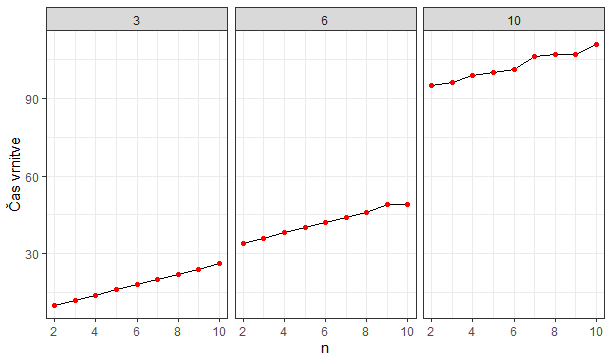
\includegraphics[width=\textwidth]{vrnitevfiksenm.png}
\end{figure}

\begin{figure}[h]
    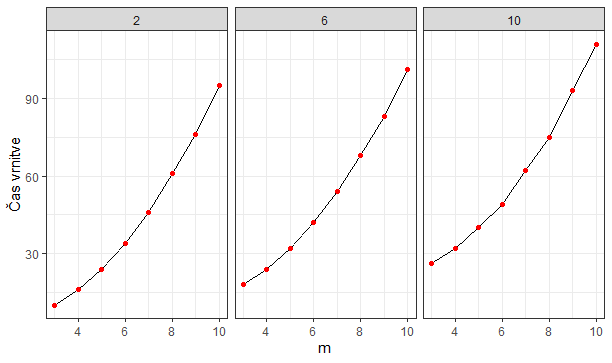
\includegraphics[width=\textwidth]{vrnitevfiksenn.png}
\end{figure}

Z $n$-jem se čas veča linearno, z $m$-jem pa kvadratično. Pričakovani čas vrnitve je približno $\mathcal{O}(m^2+n)$

\section{Primerjava grafov}

Primerjala sva različne tipe časov pri grafu lizike, grafu sonca in grafu s kliko na obeh koncih poti.
Graf sonca dobimo, če na vsako vozlišče na kliki dodamo pot dolžine $n$, graf s kliko na obeh koncih poti pa, če grafu lizike
dodamo še eno kliko na koncu poti.

\subsection{Čas pokritja}

Najprej sva primerjala čas pokritja. Graf sonca ima največji čas, kar je pričakovano, saj veliko poti zelo 
povečuje čas pokritja, kljub temu, da imamo na poti samo dve izbiri za naslednje vozlišče. Presentilo naju je,
da se čas pokritja ne poveča toliko, če dodamo grafu lizike na konec poti še eno kliko, saj se veliko časa porabi ravno na kliki, 
ker imamo toliko izbir za naslednji korak. Spodnji graf prikazuje, kako se spreminjajo ti časi glede na izbrane $n$.

\begin{figure}[h]
  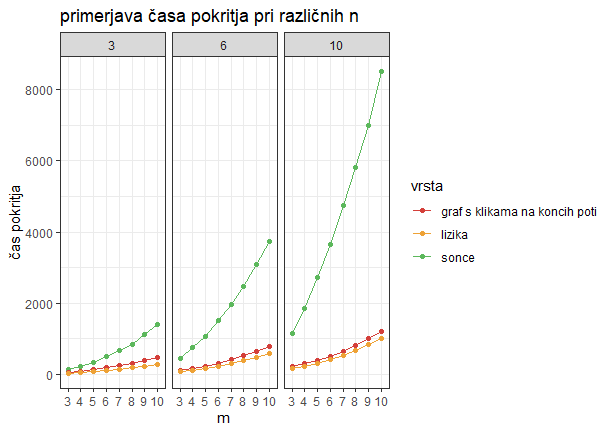
\includegraphics[width=\textwidth]{primerjava_pokritje_n.png}
\end{figure}

Če fiksirava še $m$, zopet izstopajo časi pri grafu sonca, ki se zelo hitro povečujejo. 
To prikazuje spodnji graf. Še enkrat bi poudarila, da je pomembno v katerem 
vozlišču začneva. Hitro sva ugotovila, da je pri vseh treh grafih najbolj smiselno, da začneva na kliki. Glede na analizo, ki sva jo naredila,
sva ocenila, da je čas pokritja za sonce $\mathcal{O}(n^2m^2)$, za graf lizike pa je bil $\mathcal{O}(m^2n)$. To je smiselno, saj 
se čas pokritja za graf sonca res hitreje povečuje kot pri ostalih dveh grafih. Za graf s klikama na obeh koncih poti, 
sva opazila, da se čas pokritja povečuje podobno kot čas pokritja pri grafu lizike, zato sklepava, da je čas pokritja v tem grafu enak
$\mathcal{O}(m^2n)$.

\begin{figure}[h]
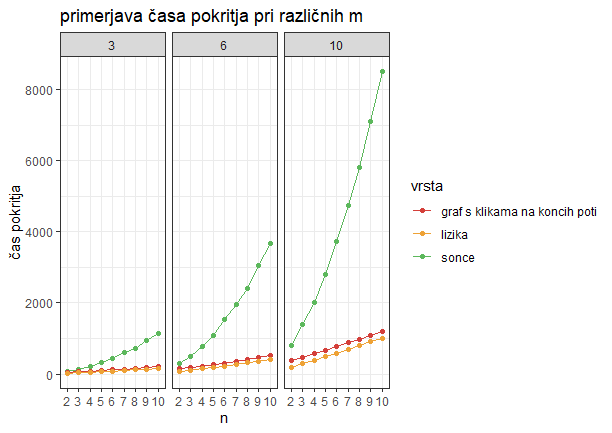
\includegraphics[width=\textwidth]{primerjava_pokritje_m.png}
\end{figure}

Ogledala sva si še, kaj se zgodi, če izbereva napačno vozlišče na začetku. Na spodnjem grafu je prikazano, kakšni so časi, če 
fiksirava $m$. Pri grafu sonca ni tako velikih sprememb, le časi nekoliko počasneje naraščajo. Pri ostalih dveh grafih, so pa časi
nižji, kot če izbereva vozlišče na kliki. Opaziva tudi, da se čas pokritja za graf s kliko na obeh koncih drugače povečuje kot se je prej.
V tem primeru ni podobno grafu liziki.

\begin{figure}[h]
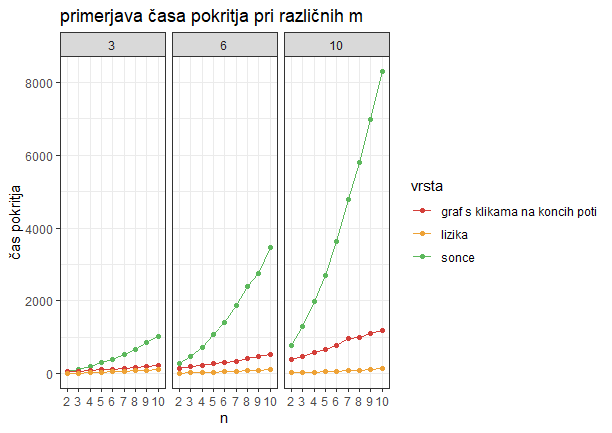
\includegraphics[width=\textwidth]{napacna_pokritje_m.png}
\end{figure}

\subsection{Čas dosega}
\subsubsection{Vozlišča v kliki}

Pri analizi grafa lizike sva ločila primere, glede na to ali je vozlišče na polnem grafu del mostu. Pri soncu
tega ni bilo potrebno narediti, saj so vsa vozlišča v kliki del mostu. Če pa grafu lizike dodava še kliko na drugem koncu poti,
morava zopet ločiti primere, ali je vozlišče del mostu ali ne.

Spodnja dva grafa prikazujeta kako sta se spreminjala časa dosega pri grafu lizike in grafu s kliko na koncih poti, kjer 
sva za začetno vozlišče izbrala vozlišče, ki ni del mostu, najprej
v odvisnosti od $m$ in pri fiksnem $n$, nato še obratno. 

\begin{figure}[h]
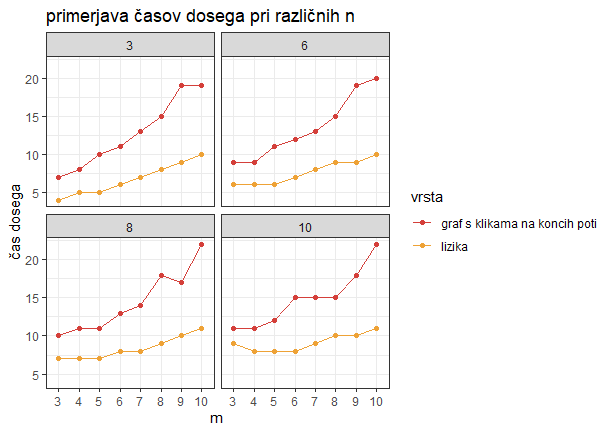
\includegraphics[width=\textwidth]{primerjava_doseg_n.png}
\end{figure}

\begin{figure}[h]
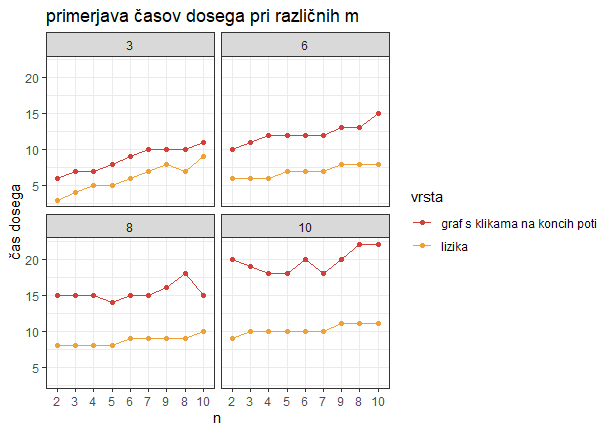
\includegraphics[width=\textwidth]{primerjava_doseg_m.png}
\end{figure}

Ko je $n$ fiksen, se čas dosega pri grafu z dvema klikama pri velikih $m$ hitreje povečuje, vendar
še vedno linearno, kot pri grafu lizike. 
Pri fiksnem $m$, pa je čas dosega skoraj neodvisen za velike klike ob spreminjanju $n$. Ker se vrednosti pri obeh
grafih spreminjajo skoraj enako, le da so pri grafu z dvema klikama nekoliko večje lahko sklepava, da je čas dosega
za ta graf enak kar času dosega grafa lizike, tj. $\mathcal{O}(m+\log(n))$.

Naprej sva analizirala, kakšen je čas dosega, če spremeniva začetno vozlišče. V naslednjem primeru je torej 
začetno vozlišče del mostu, še vedno pa je končno del klike. Spodnji graf prikazuje, kako se je spreminjal čas dosega, če fiksirava
$n$. Pričakovala sva, da bodo za oba grafa zopet podobni rezultati, vendar se čas dosega za graf z dvema klikama bistveno hitreje
povečuje. Razlog bi morda bil, ker sva začela na vozlišču ob mostu, je v naslednjem koraku z  verjetnostjo $0,5$ na poti in 
se lahko hitro zgodi, da pride do druge klike, kar pa močno poveča čas, da se vrne na prvotno kliko in potem še tam do 
končnega vozlišča.

\begin{figure}[h]
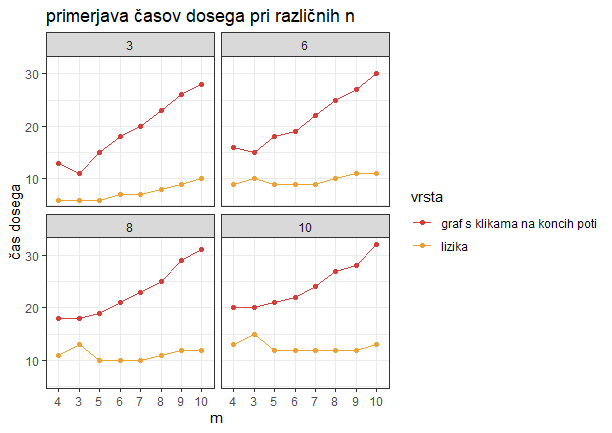
\includegraphics[width=\textwidth]{primerjava_doseg1_n.png}
\end{figure}

Da bova lahko ocenila dejanski čas dosega, si morava pogledati še, kako se spreminja čas, če fiksirava $m$. To je razvidno iz spodnjega
grafa. V tem primeru, so vrednosti pri grafu z dvema klikama višje, spreminjajo pa se podobno kot pri grafu lizike.
Napisala sva že, da je čas dosega za graf lizike v tem primeru tudi $\mathcal{O}(m+\log(n))$, za graf s klikama na obeh koncih poti
pa se spremeni na $\mathcal{O}(mn)$.

\begin{figure}[h]
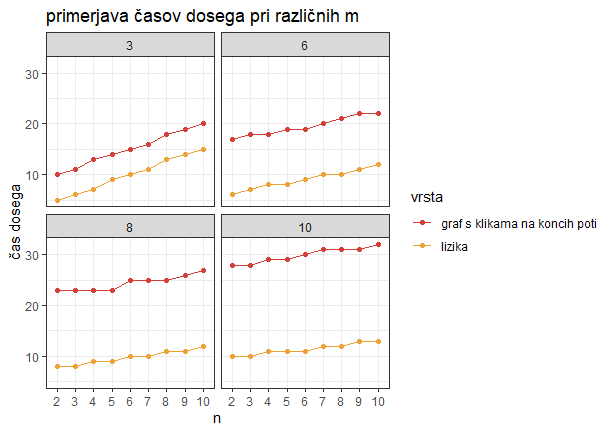
\includegraphics[width=\textwidth]{primerjava_doseg1_m.png}
\end{figure}

\subsubsection{Od vrha do dna in obratno}

Tu sva si izbrala začetno vozlišče na kliki, ki ni del mostu in pa končno na koncu poti. V tem primeru lahko primerjava
graf lizike in graf s kliko na obeh koncih poti, saj je čas dosega enak v obeh primerih. Torej je v tem primeru za oba grafa
čas dosega $\mathcal{O}(m^2n)$. če pogledava še obratno in sicer, da začneva na koncu poti in končava na kliki. V tem primeru se lahko zgodi,
da pri grafu z dvema klikama, že na začetku izberemo vozlišče, tako da se približamo drugi kliki. Sklepava, da bi bil v tem primeru,
čas dosega večji in bi se drugače spreminjal kot pri grafu lizike.

\subsection{Čas vrnitve}

Za konec sva primerjala še čas vrnitve v začetno vozlišče pri grafu lizike in grafu s kliko na obeh koncih poti. 
Zopet bova ločila primere, glede na to, ali je vozlišče v kliki in del mostu ali ni del mostu.

\subsubsection{Vozlišče v kliki, ki ni del mostu}
Pri grafu lizike sva dobila zelo podobne rezultate kot pri času dosega, ko nisva izbrala začetnega vozlišča na mostu. 
Preverila sva, da pri grafu s klikama na obeh koncih dobiva zelo podobne čase vrnitve kot pri grafu lizike, zgolj
nekoliko večje, gibajo pa se podobno. Sledi, da je tudi končna ocena v tem primeru za čas vrnitve enaka.

\subsubsection{Vozlišče v kliki, ki je del mostu}
Pri grafu lizike so bili rezultati zelo podobni kot v prejšnjem primeru, zato sklepava, da bodo tudi pri grafu z dvema klikava.
To sva tudi preverila in je res tako. Edina razlika je, da so zopet nekoliko višji. Torej je v obeh primerih čas vrnitve enak
$\mathcal{O}(m+\log(n))$.

\subsubsection{Vozlišče na koncu poti}

V tem primeru bo prišlo do razlik med grafoma, saj je pri grafu s klikama $50 \%$ možnosti, da gremo v kliko in potem šele nazaj v 
začetno vozlišče. Pričakujeva, da se bo čas vrnitve zaradi tega povečal ob fiksnem $n$, saj se bo s tem povečevala klika in posledično
bomo potrebovali dlje časa, da pridemo v začetno vozlišče. Ob fiksnem $m$ pa pričakujeva, da ne bo večjih sprememb. 
Te ugotovitve prikazujeta spodnja grafa.

\begin{figure}[h]
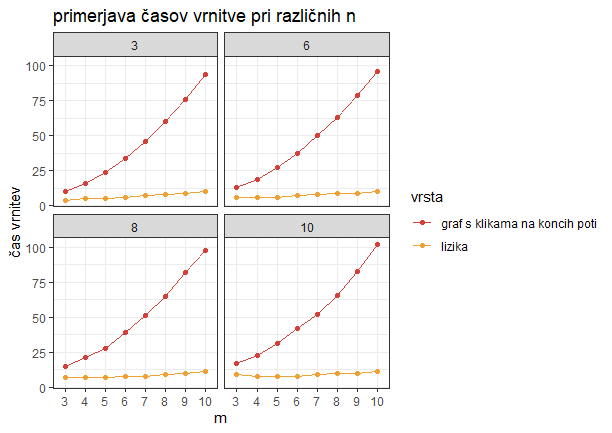
\includegraphics[width=\textwidth]{vrnitev_n.png}
\end{figure}

Kljub temu, da sva pričakovala višji čas, ko se $m$ povečuje, sva bila presenečena, da bo razlika tako velika.

\begin{figure}[h]
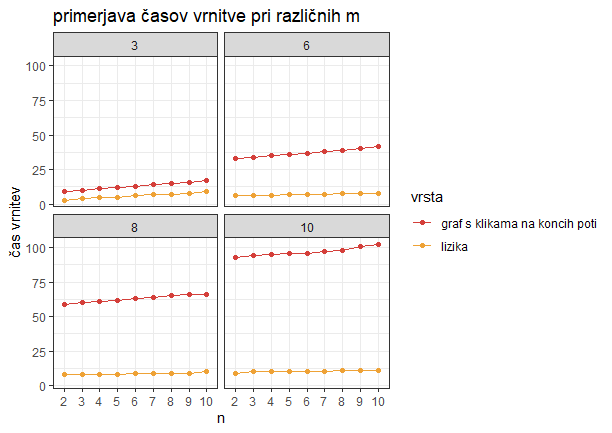
\includegraphics[width=\textwidth]{vrnitev_m.png}
\end{figure}

Na zgornjem grafu se nama je zdelo zanimivo, da je čas vrnitve pri večji $m$ bistveno večji kot pri manjših. Pri grafu lizike
ni velikih razlik, ko spreminjamo $m$. Pri $m=3$ je zelo mala razlika med časoma vrnitve pri obeh grafih. Razlog za to je, da je 
klika majhna in hitro pridemo nazaj v začetno vozlišče.



\end{document}
